\documentclass[9pt]{beamer}

\usepackage[utf8]{inputenc}

\usepackage{longtable}
\usepackage{booktabs}

\usepackage{graphicx}
\usepackage{subfig}
\usepackage{floatrow}
\captionsetup{labelsep=period}

\usepackage{tikz}
\usetikzlibrary{arrows}

\graphicspath{{./images/logos/}{./images/samples/}}

\usetheme{default}
\useinnertheme[shadow]{rounded}

%\useoutertheme[left,hideothersubsections]{IGNsidebar}
\usepackage[left,hideothersubsections]{./includes/beamerouterthemeIGNsidebar}




%/usr/share/texmf/tex/latex/beamer/themes/font/beamerfontthemedefault.sty
%/usr/share/texmf/tex/latex/beamer/themes/font/beamerfontthemeprofessionalfonts.sty
%/usr/share/texmf/tex/latex/beamer/themes/font/beamerfontthemeserif.sty
%/usr/share/texmf/tex/latex/beamer/themes/font/beamerfontthemestructurebold.sty
%/usr/share/texmf/tex/latex/beamer/themes/font/beamerfontthemestructureitalicserif.sty
%/usr/share/texmf/tex/latex/beamer/themes/font/beamerfontthemestructuresmallcapsserif.sty
\usefonttheme{structurebold}

\RequirePackage{tikz}

\definecolor{IGNVert}{RGB}{148, 192,  22}
\definecolor{IGNGris}{RGB}{112, 119, 122}

\definecolor{IGNRouge}{RGB}{255, 100, 100}

%PUCES
\setbeamercolor{item projected}{bg=IGNGris!70}

%%%%%%%%%%%%%%%%%%%%%%%%%%%%%%%%%%%%%%%%%%%%%%%%%%% COLOR
\setbeamercolor*{normal text}{fg=IGNGris}

\setbeamercolor{title}{fg=IGNGris}
\setbeamercolor{subtitle}{fg=IGNVert}
\setbeamercolor{item}{fg=IGNVert}

\setbeamercolor{caption name}{ fg=IGNGris}

\setbeamercolor{author in head/foot}{ fg=IGNGris}
\setbeamercolor{institute in head/foot}{fg=IGNGris}
\setbeamercolor{title in head/foot}{ fg=IGNGris}
\setbeamercolor{date in head/foot}{ fg=IGNGris}
\setbeamercolor{page in head/foot}{ fg=IGNGris}
\setbeamercolor{section in toc}{ fg=IGNGris}
\setbeamercolor{subsection in toc}{ fg=IGNGris}

\setbeamercolor*{block title alerted}{bg=IGNRouge!70}
\setbeamercolor*{block body alerted}{bg=IGNRouge!20}

\setbeamercolor*{block title example}{bg=IGNVert!70}
\setbeamercolor*{block body example}{bg=IGNVert!20}

\setbeamercolor*{block title}{bg=IGNGris!50}
\setbeamercolor*{block body}{bg=IGNGris!20}

%%%%%%%%%%%%%%%%%%%%%%%%%%%%%%%%%%%%%%%%%%%%%%%%%%% NAVIGATION SYMBOLS
\setbeamertemplate{navigation symbols}{}
%%%%%%%%%%%%%%%%%%%%%%%%%%%%%%%%%%%%%%%%%%%%%%%%%%% SIDE BAR
\setbeamersize{sidebar width left=1.2cm}
\setbeamercolor{section in sidebar}{fg=IGNGris}
\setbeamercolor{subsection in sidebar}{fg=IGNGris}

\setbeamercolor{section in sidebar shaded}{fg=IGNVert}
\setbeamercolor{subsection in sidebar shaded}{fg=IGNVert}


\defbeamertemplate*{sidebar}{SSB}{}

%%%%%%%%%%%%%%%%%%%%%%%%%%%%%%%%%%%%%%%%%%%%%%%%%%% HEAD LINE
\defbeamertemplate*{frametitle}{}{
  \begin{tikzpicture}[scale=0.503]
  \filldraw[color=white] (0,0) rectangle(0.1,0.54);
  \end{tikzpicture}

    \textcolor{IGNGris}{ \textbf{\insertframetitle}}
  
\begin{tikzpicture}
  \draw[very thick,color=IGNVert] (0,1)--(\paperwidth- 2.24,1);
  \end{tikzpicture}
}
%%%%%%%%%%%%%%%%%%%%%%%%%%%%%%%%%%%%%%%%%%%%%%%%%%% HEAD LINE
%\defbeamertemplate*{headline}{AH}{
%}

\defbeamertemplate*{headline}{}{}
%%%%%%%%%%%%%%%%%%%%%%%%%%%%%%%%%%%%%%%%%%%%%%%%%%% BACKGROUND

%%%%%%%%%%%%%%%%%%%%%%%%%%%%%%%%%%%%%%%%%%%%%%%%%%% FOOT LINE
\defbeamertemplate*{footline}{}
{
\leavevmode%
  \begin{tikzpicture}
  \draw (0,0) node  {};
  \draw (0.5,0) node[right]  { \textcolor{IGNGris}{\insertshorttitle}};
  \draw (5,0) node[right]  { \textcolor{IGNVert}{$\blacksquare$} \textcolor{IGNGris}{\insertshortdate{} } };
  \draw (7.5,0) node  { \textcolor{IGNVert}{$\blacksquare$} \textcolor{IGNGris}{\insertframenumber{} / \inserttotalframenumber\hspace*{2ex} }};
  \draw (9.75,0) node  { \textcolor{IGNGris}{ \insertinstitute }};
  \draw (12,0) node[right] { 
\includegraphics[height=0.25cm]{ign_logo_bottom} };
  \end{tikzpicture}

}%


%%%%%%%%%%%%%%%%%%%%%%%%%%%%%%%%%%%%%%%%%%%%%%%%%%% AT BEGIN SECTION


\AtBeginSection[]
{
\setbeamercolor{section in sidebar}{fg=white }
\setbeamercolor{subsection in sidebar}{fg=white }

\setbeamercolor{section in sidebar shaded}{fg=white }
\setbeamercolor{subsection in sidebar shaded}{fg=white }



\begin{frame}{
  
\begin{tikzpicture}[scale=0.503]
  \draw[color=IGNGris,fill=IGNGris]  (0,0) rectangle (23,9);
  \draw (1,1) node [right,text width=10cm,text justified]  {  \textcolor{white}{\insertsection}};
  \end{tikzpicture}
}
\end{frame}


\setbeamercolor{section in sidebar}{fg=IGNGris}
\setbeamercolor{subsection in sidebar}{fg=IGNGris}

\setbeamercolor{section in sidebar shaded}{fg=IGNVert}
\setbeamercolor{subsection in sidebar shaded}{fg=IGNVert}

\addtocounter{framenumber}{-1}

}


\usepackage{standalone}

\usepackage{amssymb}
\usepackage{amsmath}
\usepackage{mathrsfs}
\usepackage{mathtools}
\usepackage{dsfont}
\usepackage{bbold}


\usepackage{pdfpages}
\usepackage{hyperref}

\usepackage{color}

%%%%%%%%%%%%%%%%%%%%%%%%%%%%%%%%%%%%%%%%%%%%%%%%%%%%%%%%%%%%%%%%%%%%%%%%%%%%%%%%%%%%%%%%%%%%%%%%%%%%%%%%%
\title{Traitements avancés des images de Télédétection}
\subtitle{SVM et Sélection d'attribut}
\author{Oussama ENNAFII}
\institute{ENSG}
\date{\today}

%%%%%%%%%%%%%%%%%%%%%%%%%%%%%%%%%%%%%%%%%%%%%%%%%%%%%%%%%%%%%%%%%%%%%%%%%%%%%%%%%%%%%%%%%%%%%%%%%%%%%%%%%
\AtBeginSubsection[]
{
	\begin{frame}<beamer>
		\frametitle{Presentation Layout}
		\tableofcontents[
		currentsection,
		sectionstyle=show/shaded,
		subsectionstyle=show/shaded/hide
		]
	\end{frame}
}

\AtBeginSection[]
{
	\begin{frame}<beamer>
		\frametitle{Presentation Layout}
		\tableofcontents[
		currentsection,
		sectionstyle=show/shaded,
		subsectionstyle=hide
		]
	\end{frame}
}

\begin{document}

	\usebackgroundtemplate{
		\begin{tikzpicture}
			\node (bg) {
				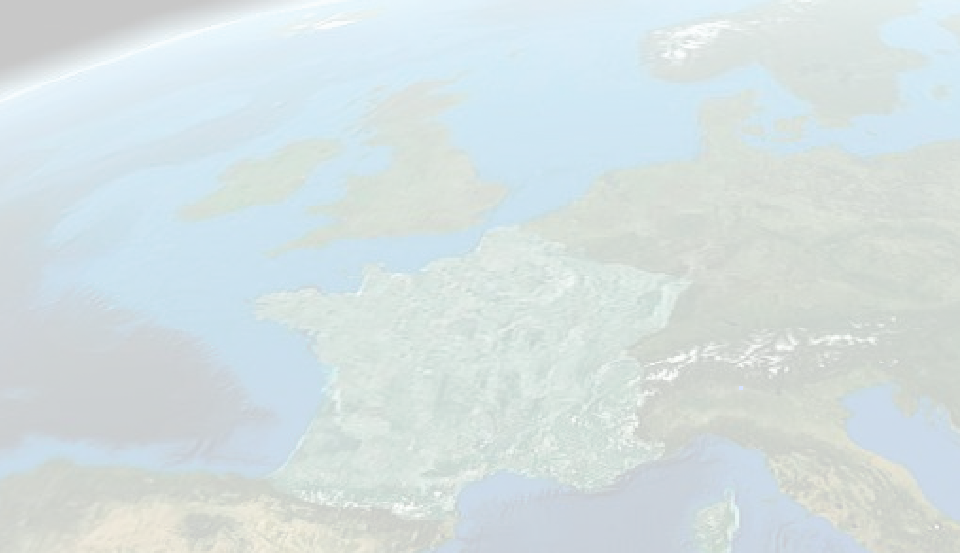
\includegraphics[width=12.5cm]{from_space_background}
			};
			\path (bg.north)+(-5.5, 1) node (ign) {
				
\includegraphics[height=1.5cm]{ign_logo}
			};
			\path (ign.east)+(10.25, 0) node {
				
\includegraphics[width=1.5cm]{ensg_logo}
			};
		\end{tikzpicture}
	}

	\begin{frame}[plain,c]
		\begin{columns}
			\begin{column}{8cm}
				\begin{center}
					\vspace{2cm}
					\titlepage{}
				\end{center}
			\end{column}
			\begin{column}{1cm}
			\end{column}
		\end{columns}
	\end{frame}

	\usebackgroundtemplate{
		
\begin{tikzpicture}[scale=0.503]
			\filldraw[color=IGNGris] (0,0) rectangle(2.62,0.54);
			\filldraw[color=IGNGris] (4.77,0) rectangle(2.62+4.77,0.54);

			\filldraw[color=IGNVert] (9.50+0.27,0) -- (9.50,0.54)-- (9.50+7.41-0.27,0.54)-- (9.50+7.41,0)--cycle;

			\filldraw[color=IGNGris] (19.50,0) rectangle(2.62+19.50,0.54);
			\filldraw[color=IGNGris] (23.11,0.54)--(23.11+0.54,0)--(2.3+23.11,0)--(2.3+23.11,0.54)--cycle;;
		\end{tikzpicture}
	}


	%%%%%%%%%%%%%%%%%%%%%%%%%%%%%%%% toc %%%%%%%%%%%%%%%%%%%%%%%%%%%%%%%%%%%%%%%
	\setbeamercolor{section in sidebar}{fg=white }
	\setbeamercolor{subsection in sidebar}{fg=white }
	\setbeamercolor{section in sidebar shaded}{fg=white }
	\setbeamercolor{subsection in sidebar shaded}{fg=white }
	\begin{frame}
			\tableofcontents
	\end{frame}
	\setbeamercolor{section in sidebar}{fg=IGNGris}
	\setbeamercolor{subsection in sidebar}{fg=IGNGris}
	\setbeamercolor{section in sidebar shaded}{fg=IGNVert}
	\setbeamercolor{subsection in sidebar shaded}{fg=IGNVert}
	%%%%%%%%%%%%%%%%%%%%%%%%%%%%%%%%%%%%%%%%%%%%%%%%%%%%%%%%%%%%%%%%%%%%%%%%%%%%

	\section*{Introduction}

	\begin{frame}{Rappel}
		\begin{figure}[H]
			\begin{center}
				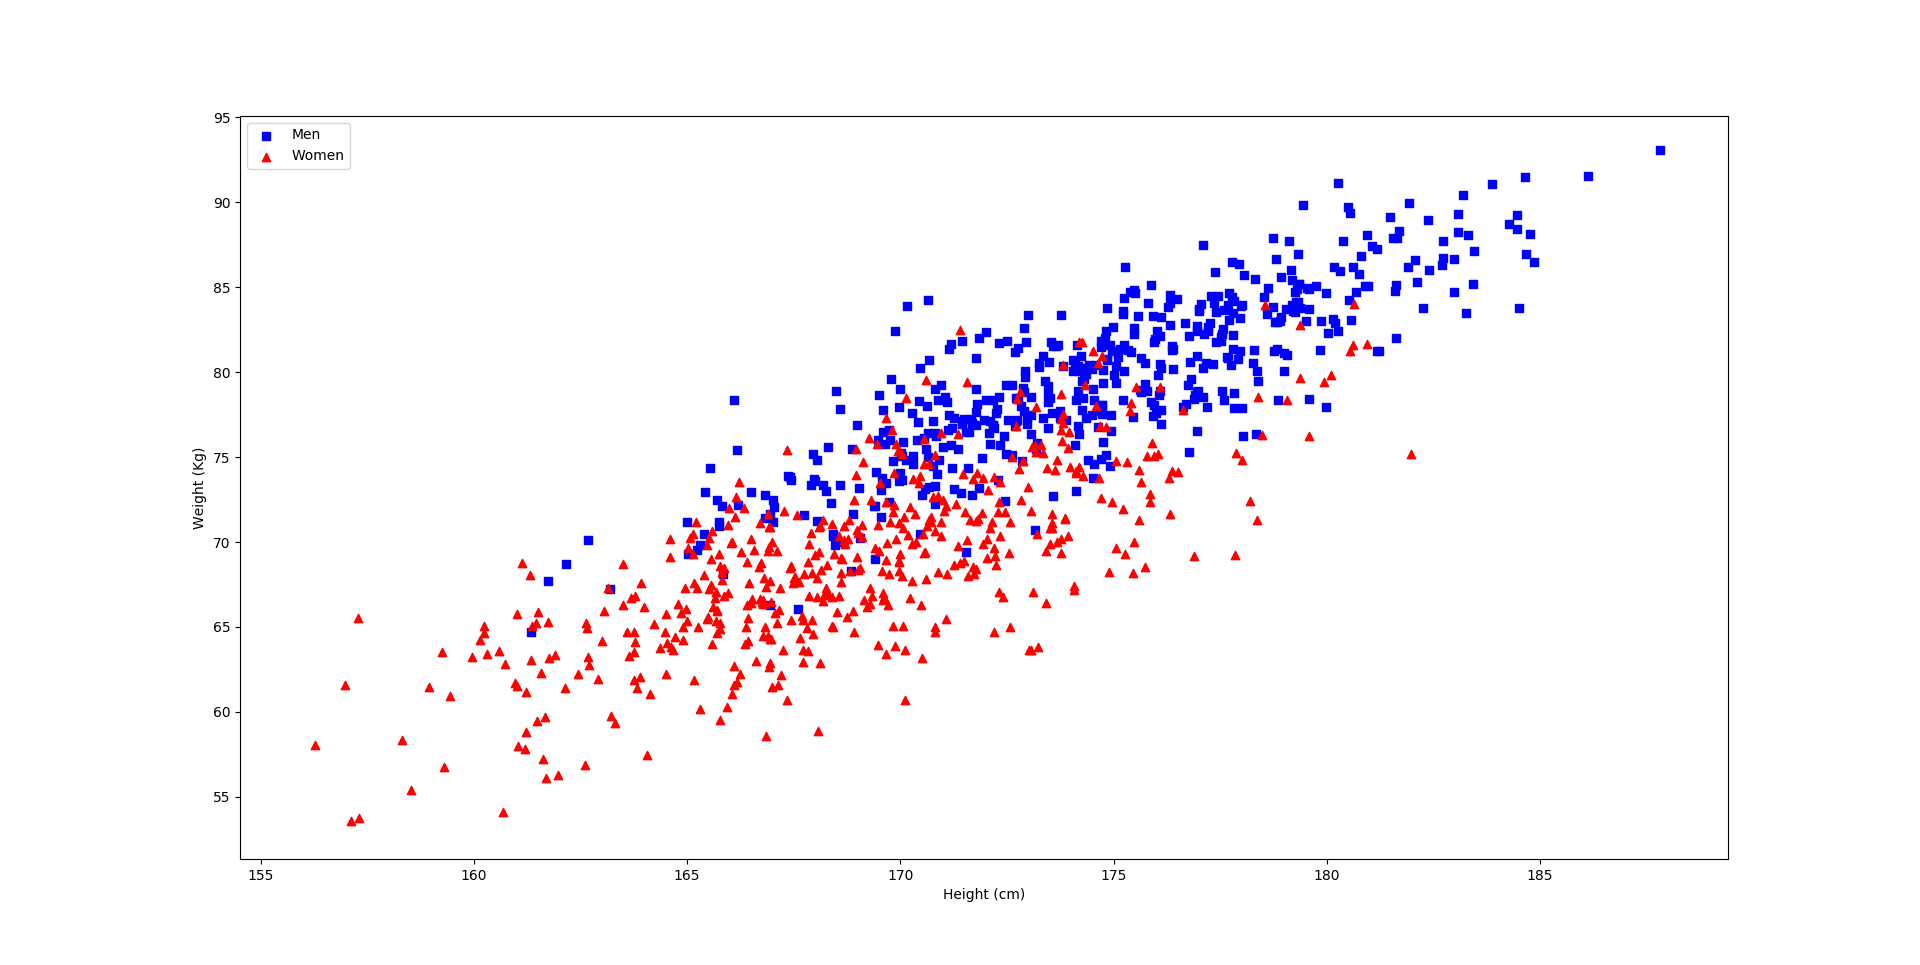
\includegraphics[width=.7\textwidth]{sample_2d}
				\caption{\label{fig::sample_2d} Example de problème de classification: $2$ attributs et $2$ classes.}
			\end{center}
		\end{figure}
		\begin{itemize}
			\item[--]<1-> On observe $n$ échantillons: $\Big((X^i, Y^i)\Big)_{i=1,\dots,n}$,
			\item[--]<2-> Sachant une instance $X^j = \begin{pmatrix}
			X_1^j\\
			\vdots \\
			X_d^j
			\end{pmatrix}$, il faut prédire sa classe $Y^j$ et sa probabilité.
		\end{itemize}
	\end{frame}

	\begin{frame}{Supervisé vs Non-Supervisée}
		\begin{figure}[H]
			\begin{center}
				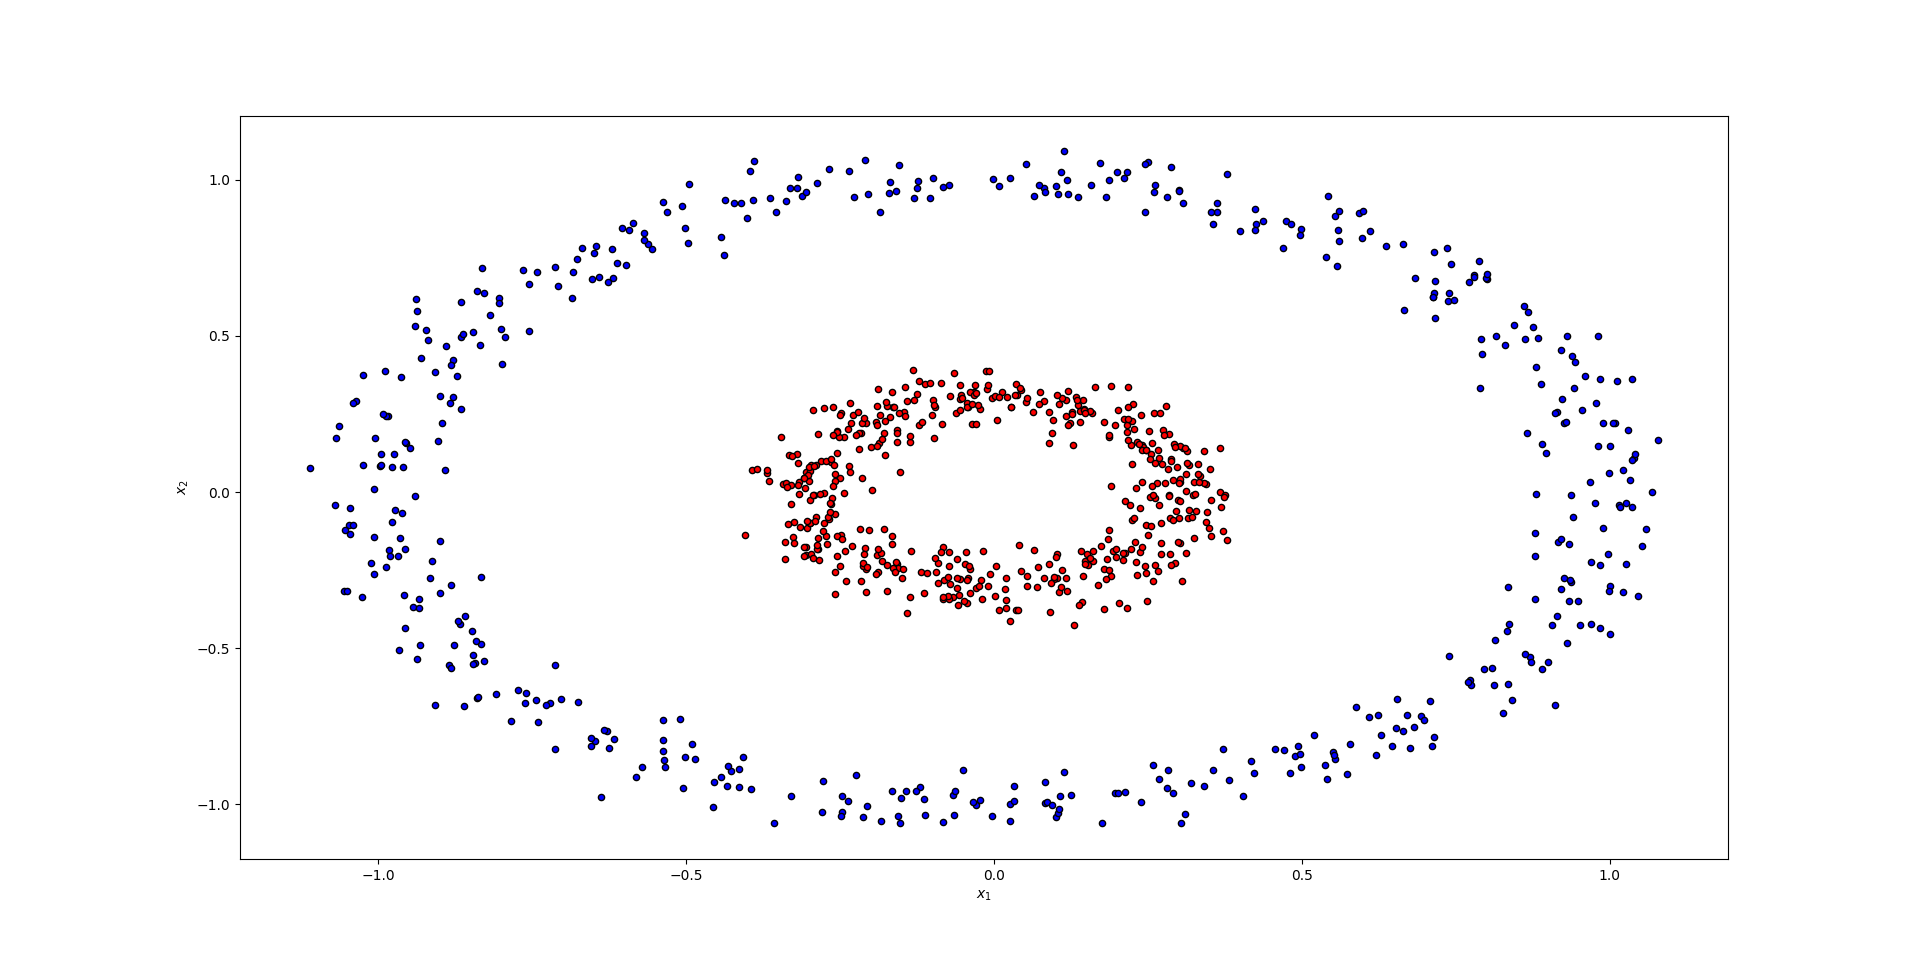
\includegraphics[width=.7\textwidth]{circles}
				\caption{\label{fig::circles} Example de problème de classification non supervisée: Pas de classes mais une structure se dégage.}
			\end{center}
		\end{figure}
		\begin{itemize}
			\item[--]<1-> On observe que les instances ${(X^i)}_{i=1,\dots,n}$ sans les classes $\longrightarrow$ Classification non supervisée,
			\item[--]<2-> On observe des instances et leurs classes respectives ${\Big((X^i, Y^i)\Big)}_{i=1,\dots,n}$ $\longrightarrow$ Classification supervisée.
		\end{itemize}
	\end{frame}

	\begin{frame}{Discriminatif vs Génératif}
		Les échantillons réalise une loi de distribution inconnues $\mathbb{P}(X^i=x,Y^i=y)=p(x,y)$ et sont indépendents entre eux. La prédiction dépend de notre connaissance préalable:
		\begin{itemize}
			\item[--]<1-> On sait modéliser la distribution des classes et la réalisation des instances selon cette classe $p(x,y) = p(y).p(x\vert y)$ $\longrightarrow$ méthode générative,
			\begin{itemize}
				\item[--]<2-> On suppose que la répartition des sexes est équilibrée dans le monde et que la répartition des mesures --- poids et taille --- suivent des lois gaussiennes (c.f Figure~\ref{fig::sample_2d});
			\end{itemize}
			\item[--]<3-> On n'a aucune connaissance \textit{a priori}. On cherche à apprendre $ p(x,y) = p(y \vert x).p(x)$ $\longrightarrow$ méthode discriminative,
			\begin{itemize}
				\item[--]<4-> On apprend un modèle d'arbres aléatoires.
			\end{itemize}
		\end{itemize}
	\end{frame}

	\begin{frame}{Pourquoi classifier?}
		\begin{figure}[H]
			\ffigbox[\FBwidth]
			{
				\begin{subfloatrow}[2]
					\ffigbox[\FBwidth]
					{
						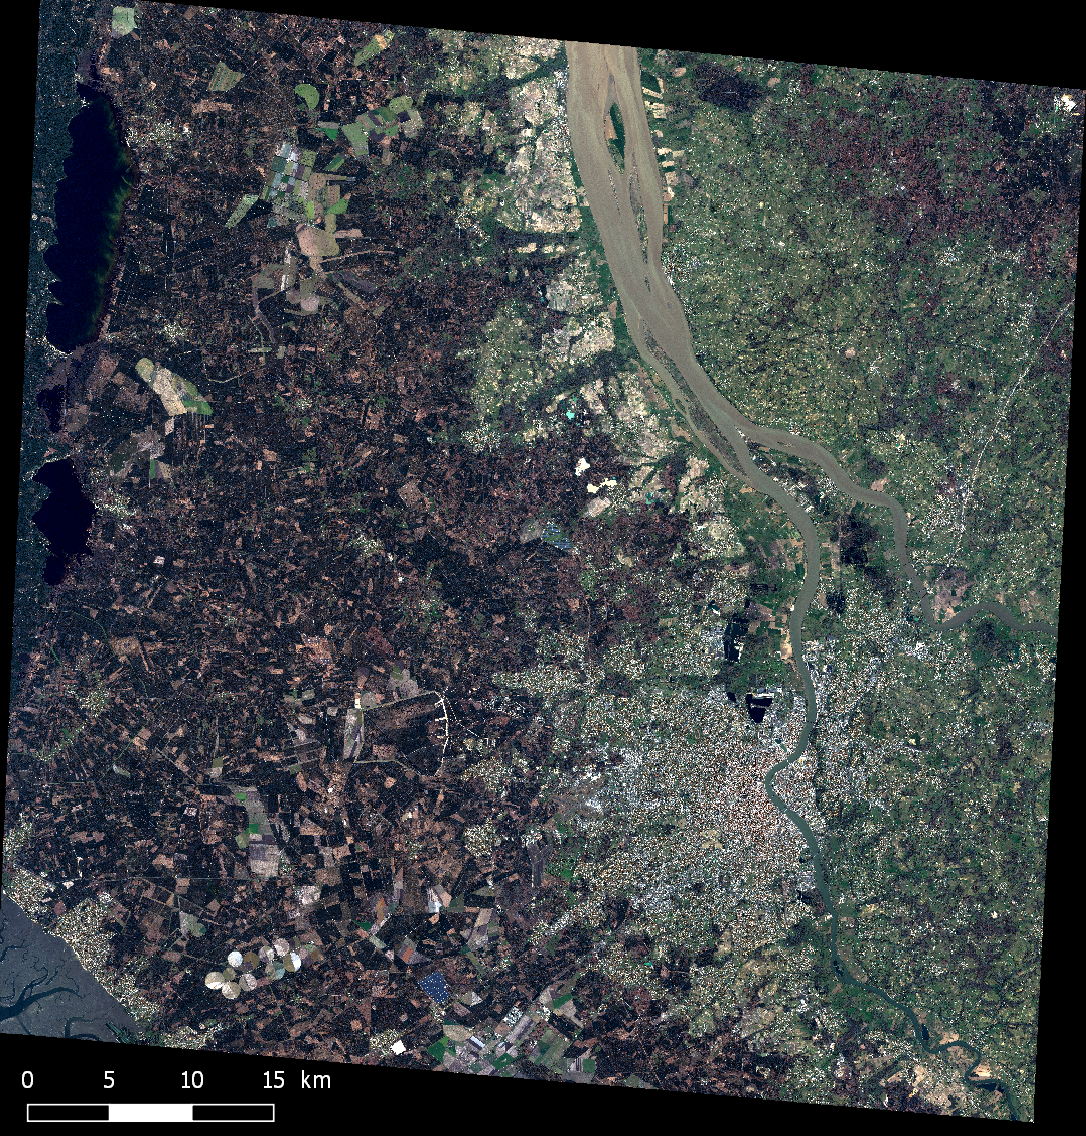
\includegraphics[width=.45\textwidth]{gironde}
					}
					{
						\caption{Image de la Gironde prise par SPOT en 2016: Résolution $1.5m$, $4$ canaux: \{{\color{purple!20}Infrarouge}, {\color{red}Rouge}, {\color{green}Vert}, {\color{blue}Bleu}\}.}\label{fig::gir}
					}
					\ffigbox[\FBwidth]
					{
						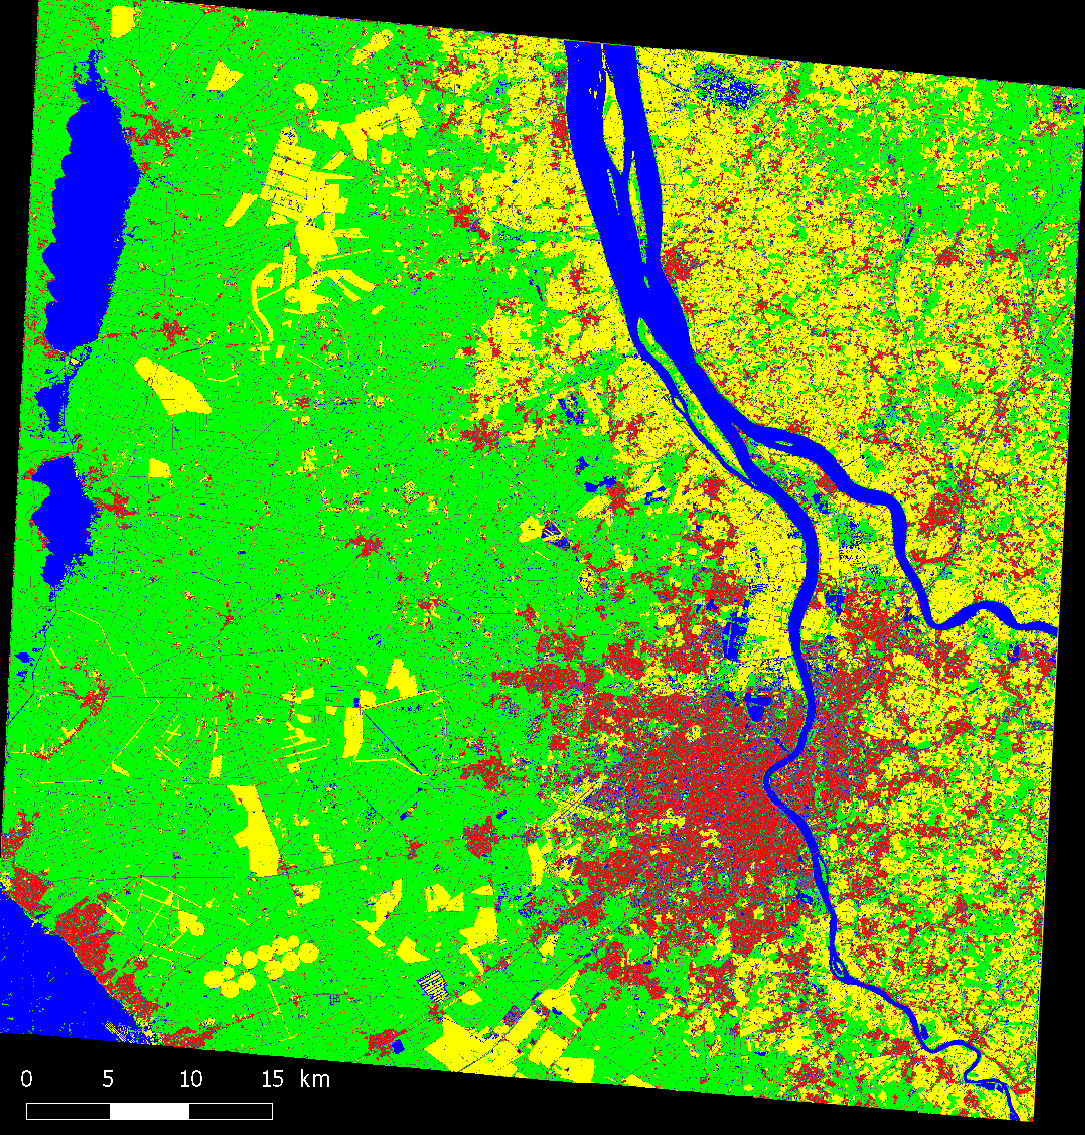
\includegraphics[width=.45\textwidth]{gironde_classif}
					}
					{
						\caption{Occupation des sols extraite de l'image: {\color{red}$\blacksquare$} Bâti, {\color{green}$\blacksquare$} Forêt, {\color{yellow}$\blacksquare$} Culture, {\color{gray}$\blacksquare$} Routes, {\color{blue}$\blacksquare$} Eau.}\label{fig::gir_ocd}
					}
				\end{subfloatrow}
			}
			{
				\caption{\label{fig::ocs} Classification appliquée pour l'Occupation des sols~\cite{postadjian2017investigating}.}
			}
		\end{figure}
	\end{frame}

	\begin{frame}{Pourquoi classifier?}
		\begin{figure}[H]
			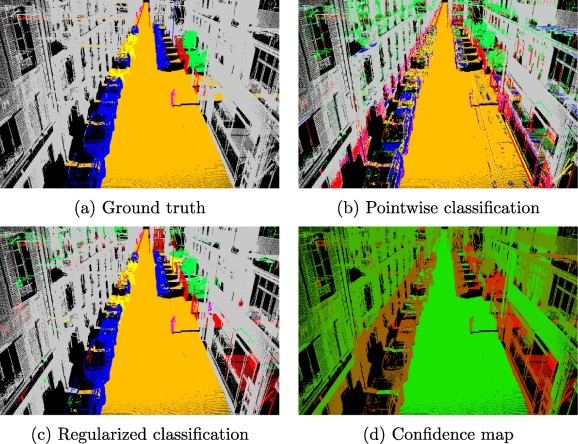
\includegraphics[width=.7\textwidth]{pc_classification}
			\caption{\label{fig::pc_classif}Example de classification de nuage de point\cite{LANDRIEU2017102}.}
		\end{figure}
	\end{frame}

	\section[SVM]{SVM}
	\begin{frame}{Curse of dimensionality}
		\begin{itemize}
			\item[--]<1-> Si on a $n$ points à séparer, sans un modèle de classification, il y a un nombre exponentiel de séparations $\sum_{k=0,\dots,\lfloor \frac{n}{2} \rfloor} \begin{pmatrix}
			n\\
			k
			\end{pmatrix} = 2^{n-1}$ qui sont possible $\longrightarrow$ C'est incalculable.
			\item[--]<2-> Il faut donc un modèle de séparation qui permettra de chercher efficacement une bonne solution: Forêts Aléatoires, \textbf{SVM}, Réseaux de Neurones \dots
		\end{itemize}
	\end{frame}
	\subsection[linear]{Séparateur linéaire}
	\begin{frame}{Mais c'est quoi donc ce SVM?}
		\begin{itemize}
			\item[--] SVM\@: Support Vector Machines;
			\item[--] C'est donc un vecteur support?
		\end{itemize}
	\end{frame}

	\begin{frame}{Séparateur}
		On se place dans le cas de classification binaires:
		$$ X^i \in \mathbb{R}^d , \quad \forall i=1,\dots,n$$
		$$ Y^i \in \{-1, +1\} , \quad \forall i=1,\dots,n$$
		\begin{itemize}
			\item[--]On cherche une fonction qui modélise la probabilité
			$$f: x \mapsto f(x) = (+1) \times p(1\vert x) + (-1) \times p(-1\vert x)$$
			à partir duquel on en déduit le décideur:
			\begin{align*}
				D: \mathbb{R}^d &\rightarrow \{-1, +1\} \\
				x &\mapsto D(x) = sign(f(x))
			\end{align*}
			\item[--] Le séparateur est la courbe qui vérifie:
			\begin{align*}
				\mathscr{S} &\triangleq \{X \in \mathbb{R}^d: f(X) = 0\} \\
							&= \{X \in \mathbb{R}^d: p(1\vert x) = p(-1\vert x)\}
			\end{align*}
		\end{itemize}
	\end{frame}

	\begin{frame}{Séparateur}
		\begin{figure}[H]
			\ffigbox[\FBwidth]
			{
				\begin{subfloatrow}[2]
					\ffigbox[\FBwidth]
					{
						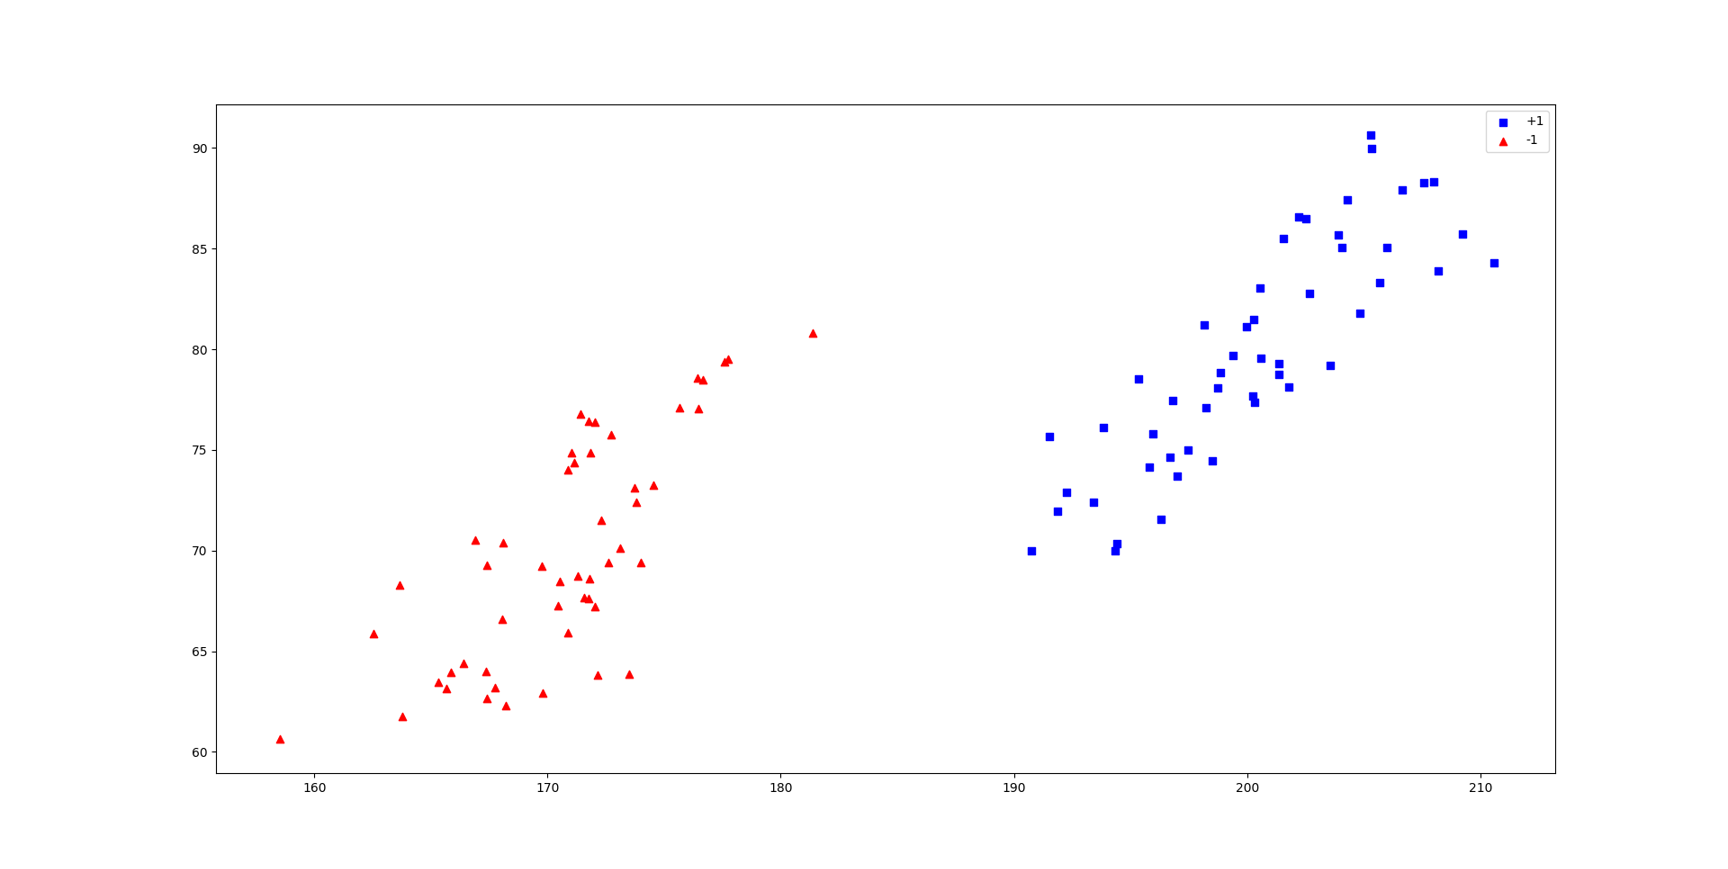
\includegraphics[width=.45\textwidth]{sample_svm}
					}
					{
						\caption{Echantillons à séparer.}\label{fig::sample_sep}
					}
					\ffigbox[\FBwidth]
					{
						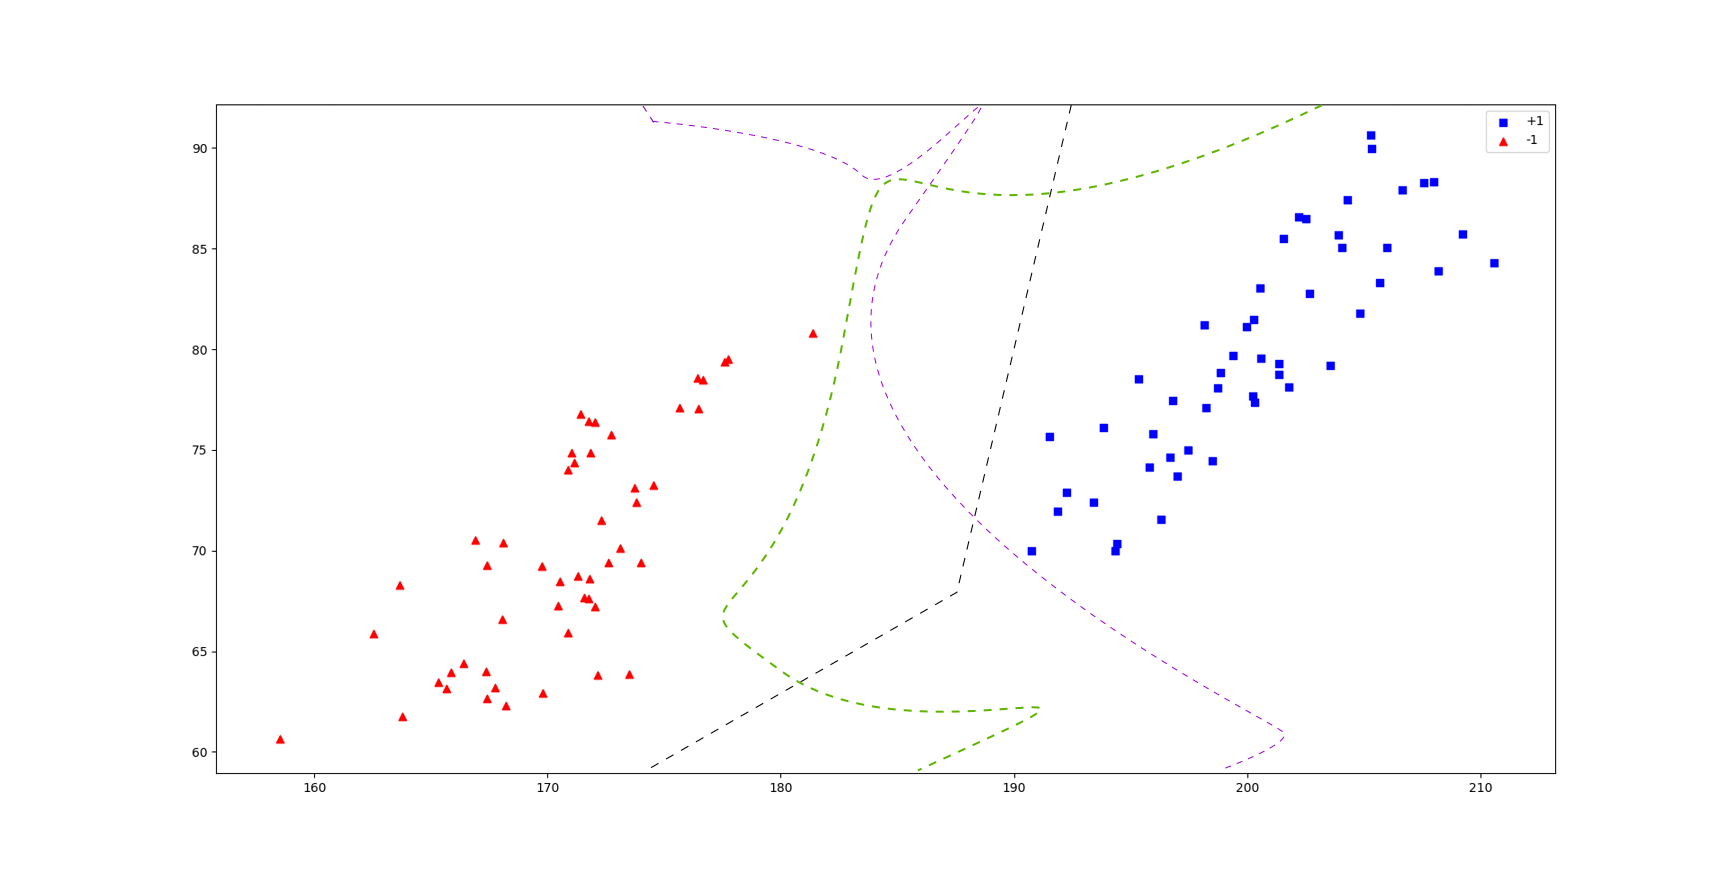
\includegraphics[width=.45\textwidth]{separators}
					}
					{
						\caption{Examples de séparateurs possible.}\label{fig::sep_ex}
					}
				\end{subfloatrow}
			}
			{
				\caption{\label{fig::separators} Example de séparation de données.}
			}
		\end{figure}
	\end{frame}

	\begin{frame}{Choix du séparateur}
		\begin{itemize}
			\item[--] Il y a une infinité de modèle de $f(X)$ possible.
			\item[--] Le choix le plus naïf serait:
			\begin{equation*}
				f = \sum_{i=1,\dots,n} Y^i . \delta_{X^i}
			\end{equation*}
			Par contre ce classifieur n'a pas de pourvoir de généralization. En effet:
			\begin{gather*}
				\widetilde{x} \leftarrow \sum_{i=1,\dots,n} X^i \notin \{X^i, \forall i=1,\dots,n\} \\
				\Rightarrow f(\widetilde{x}) = 0
			\end{gather*}
			\item[--] On s'intéresse ici au séparateur linéaire:
			\begin{align*}
				f_{\textbf{w}, b}: \mathbb{R}^d &\rightarrow \{-1, 0, +1\} \\
				\textbf{x} &\mapsto f_{\textbf{w}, b}(\textbf{x}) = \textbf{w}.\textbf{x} + b
			\end{align*}
		\end{itemize}
	\end{frame}

	\begin{frame}{Séparateur linéaire}
		\begin{figure}[H]
			\ffigbox[\FBwidth]
			{
				\begin{subfloatrow}[2]
					\ffigbox[\FBwidth]
					{
						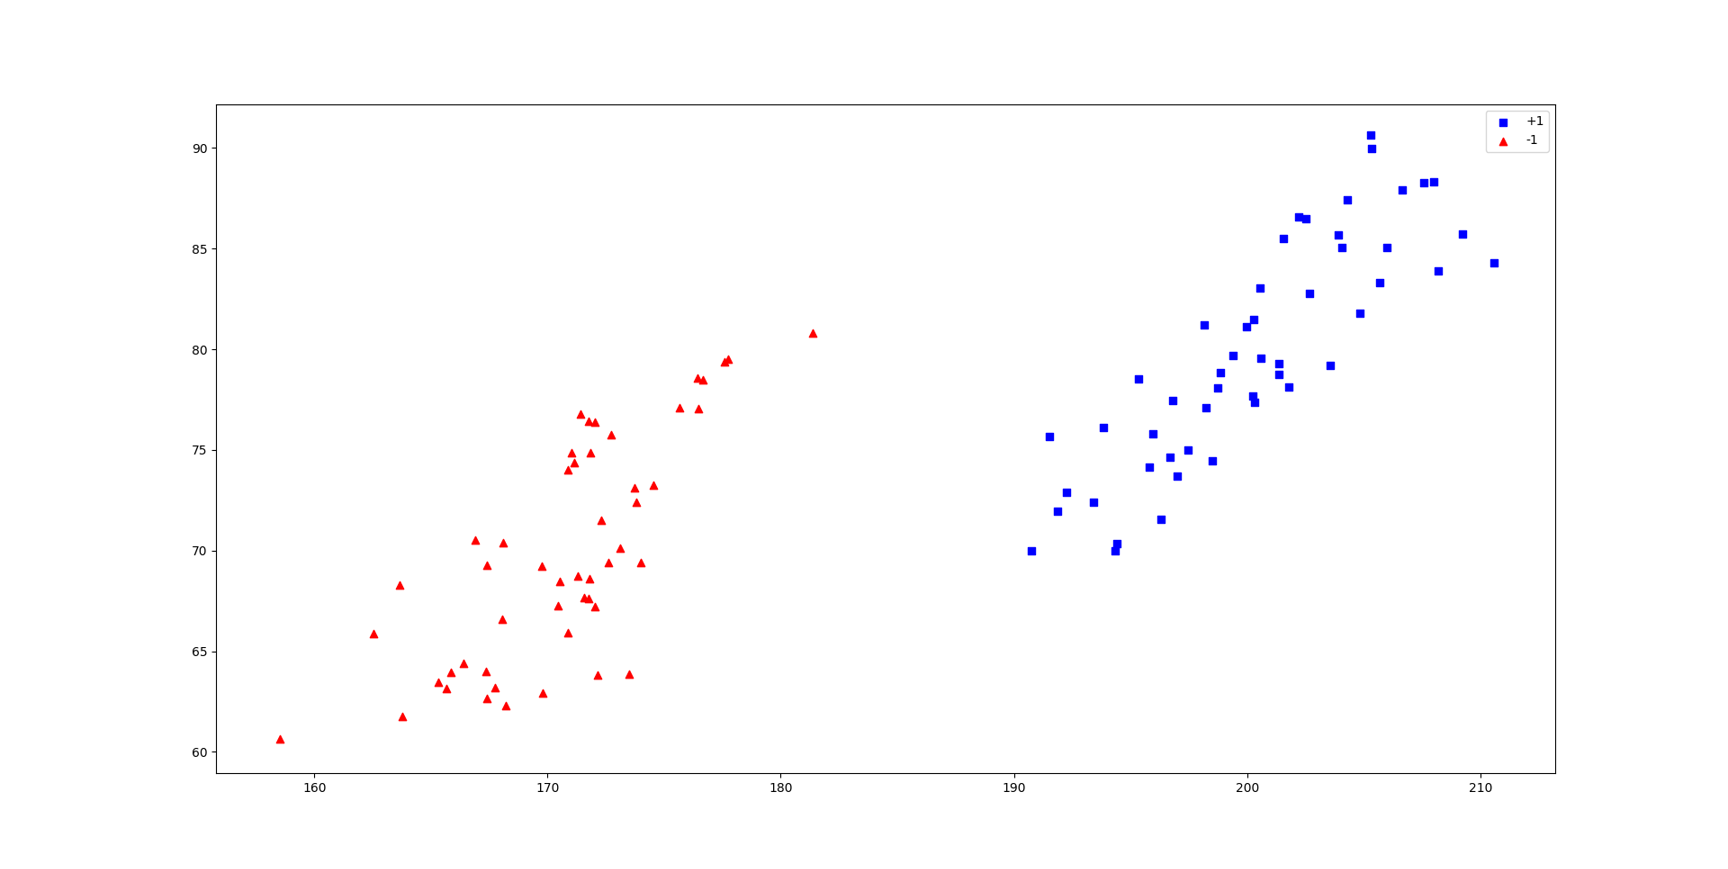
\includegraphics[width=.45\textwidth]{sample_svm}
					}
					{
						\caption{Echantillons à séparer.}\label{fig::sample_sep2}
					}
					\ffigbox[\FBwidth]
					{
						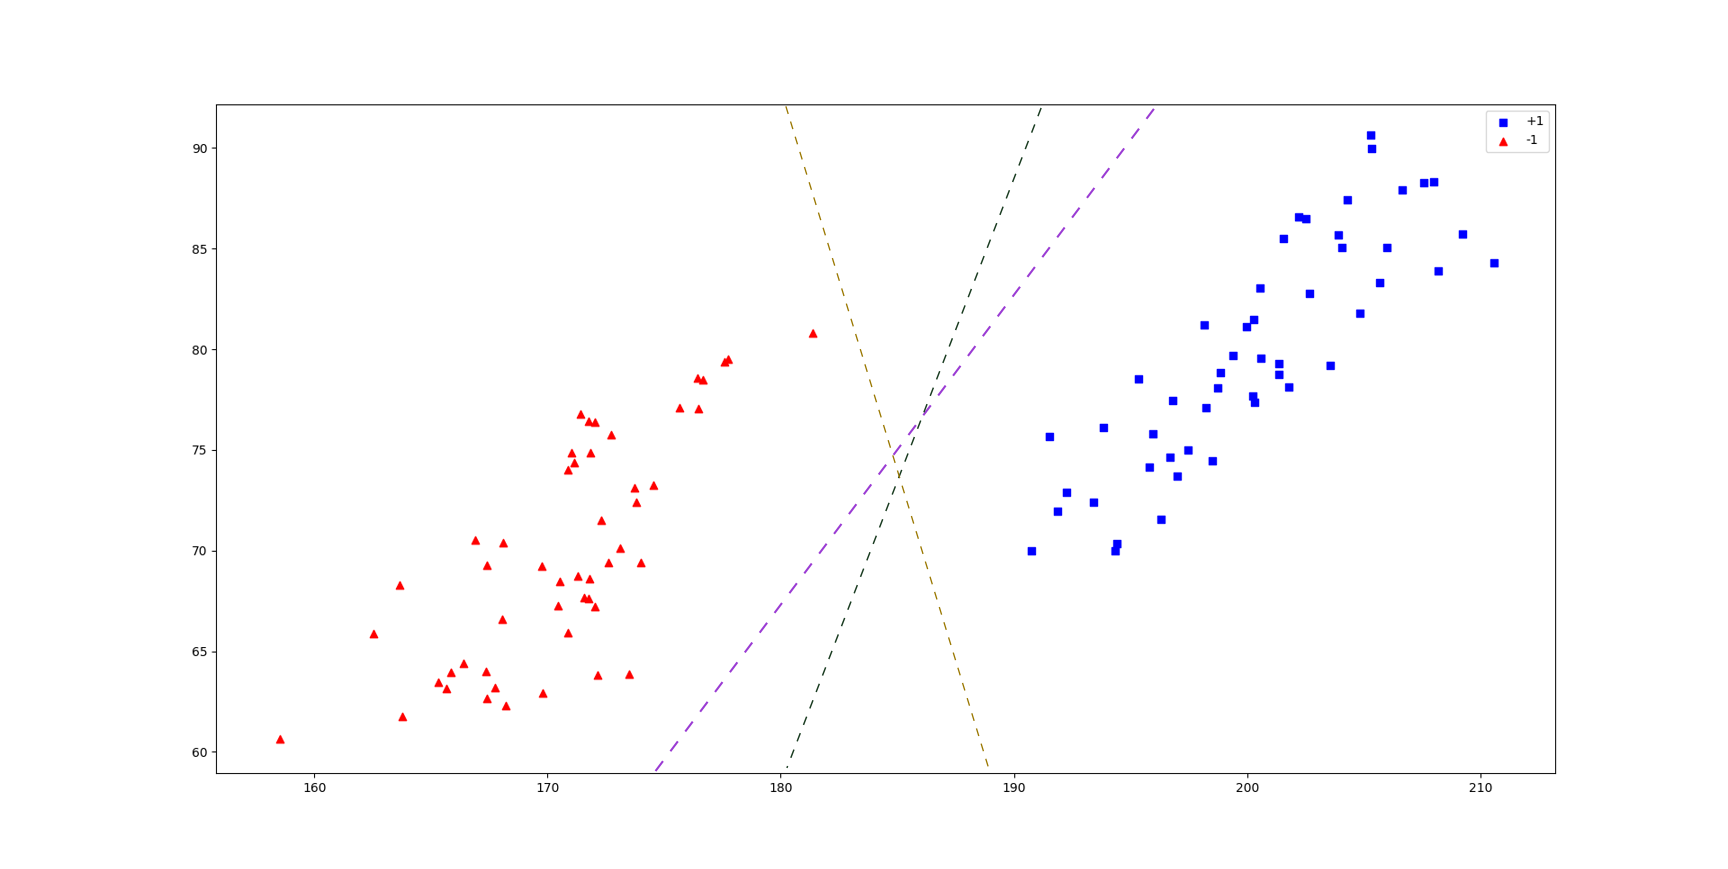
\includegraphics[width=.45\textwidth]{linear_separation}
					}
					{
						\caption{Examples de séparateurs linéaire possible.}\label{fig::lin_sep}
					}
				\end{subfloatrow}
			}
			{
				\caption{\label{fig::lin_separators} Example de séparation linéaire de données.}
			}
		\end{figure}
	\end{frame}

	\subsection[linear]{SVM linéaire}
	\begin{frame}{Mais c'est quoi donc ce SVM?}
		\begin{itemize}
			\item[--] SVM\@: Support Vector Machines.
			\item[--] C'est quoi donc un vecteur support?
			\item[--] Quelle est la relation avec les séparateurs linéaires?
		\end{itemize}
	\end{frame}

	\begin{frame}{SVM\@: maximiser la marge.}
		\begin{figure}[H]
			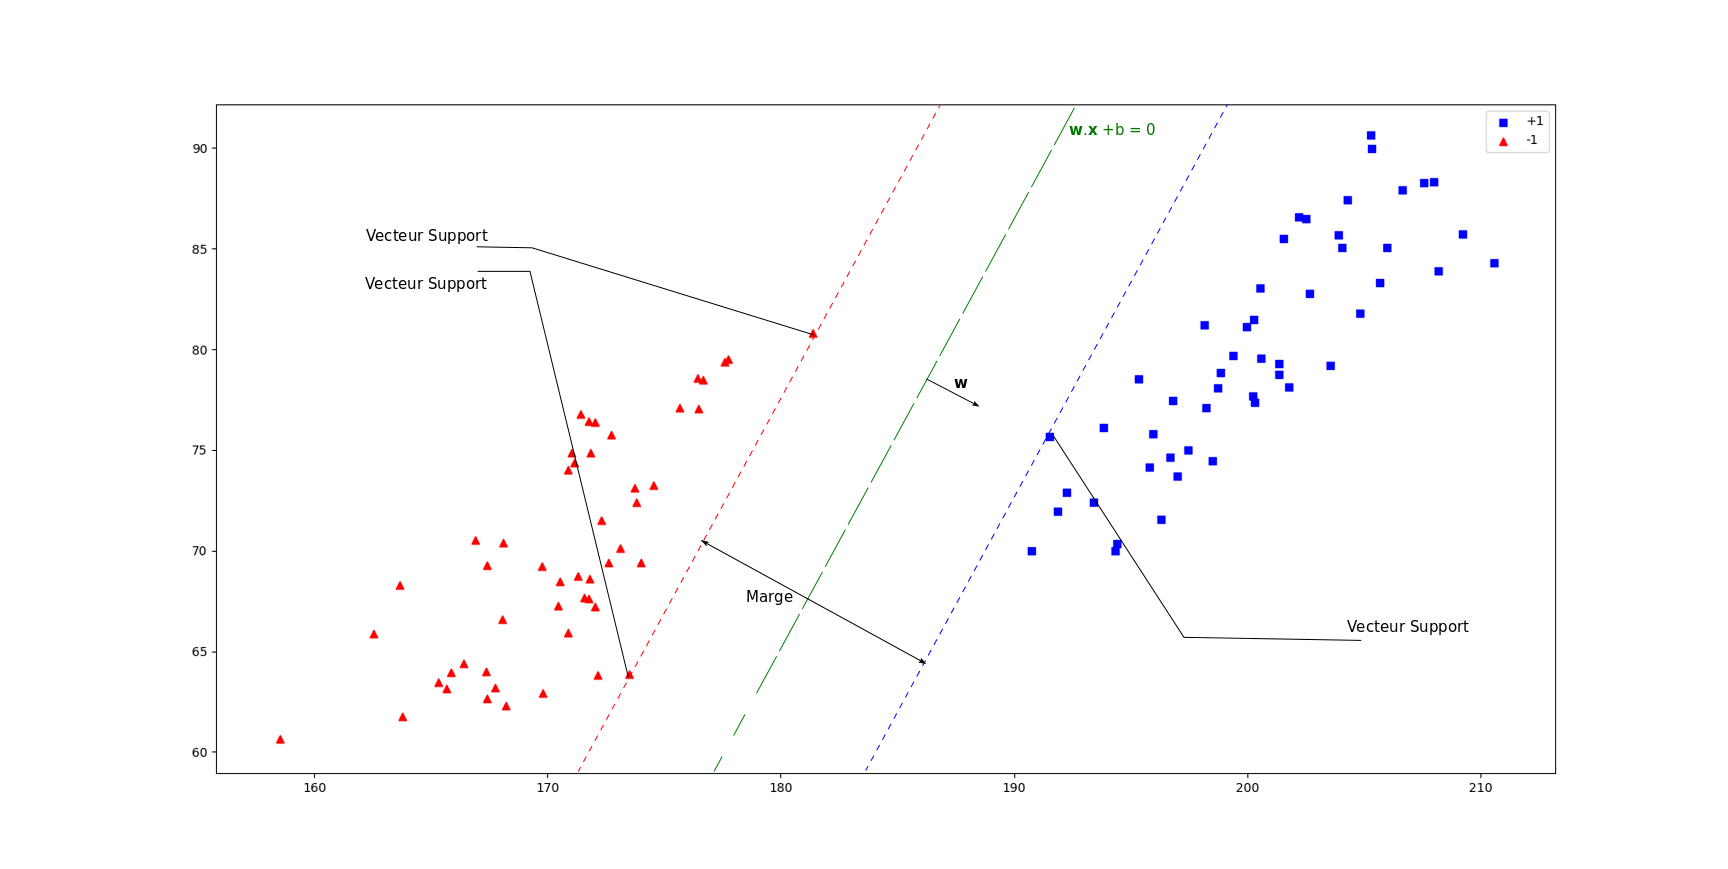
\includegraphics[width=\textwidth]{svm}
			\caption{\label{fig::svm} Le séparateur linéaire SVM.}
		\end{figure}
	\end{frame}

	\begin{frame}{SVM\@: maximiser la marge.}
		\begin{itemize}
			\item[--] Le but du SVM est de maximiser la marge~\cite{vapnik1998statistical}.
			\item[--] On remarque que:
			\begin{gather*}
				\textbf{w} \in \{\omega \in \mathbb{R}^d : f_{\omega, b} = \mathbb{0}\} \\
				\Rightarrow
				\lambda . \textbf{w} \in \{\omega \in \mathbb{R}^d : f_{\omega, b} = \mathbb{0}\}\quad, \forall \lambda \in \mathbb{R}\setminus\{0\}
			\end{gather*}
			\item[--] On prend donc la solution $\textbf{w}$ qui permet d'avoir:
			\begin{align}
				\textbf{w}.\textbf{x}_{\color{blue}+} + b &= {\color{blue}+}1 \\
				\textbf{w}.\textbf{x}_{\color{red}-} + b &= {\color{red}-}1
			\end{align}
			où:
			\begin{itemize}
				\item[{\color{blue}+}] $\textbf{x}_{\color{blue}+}$ correspond aux supports vecteurs positifs (i.e. $Y={\color{blue}+}1$).
				\item[{\color{red}---}] $\textbf{x}_{\color{red}-}$ correspond aux supports vecteurs négatifs (i.e. $Y={\color{red}-}1$).
			\end{itemize}
		\end{itemize}
	\end{frame}

	\begin{frame}{SVM\@: maximiser la marge.}
		\begin{figure}[H]
			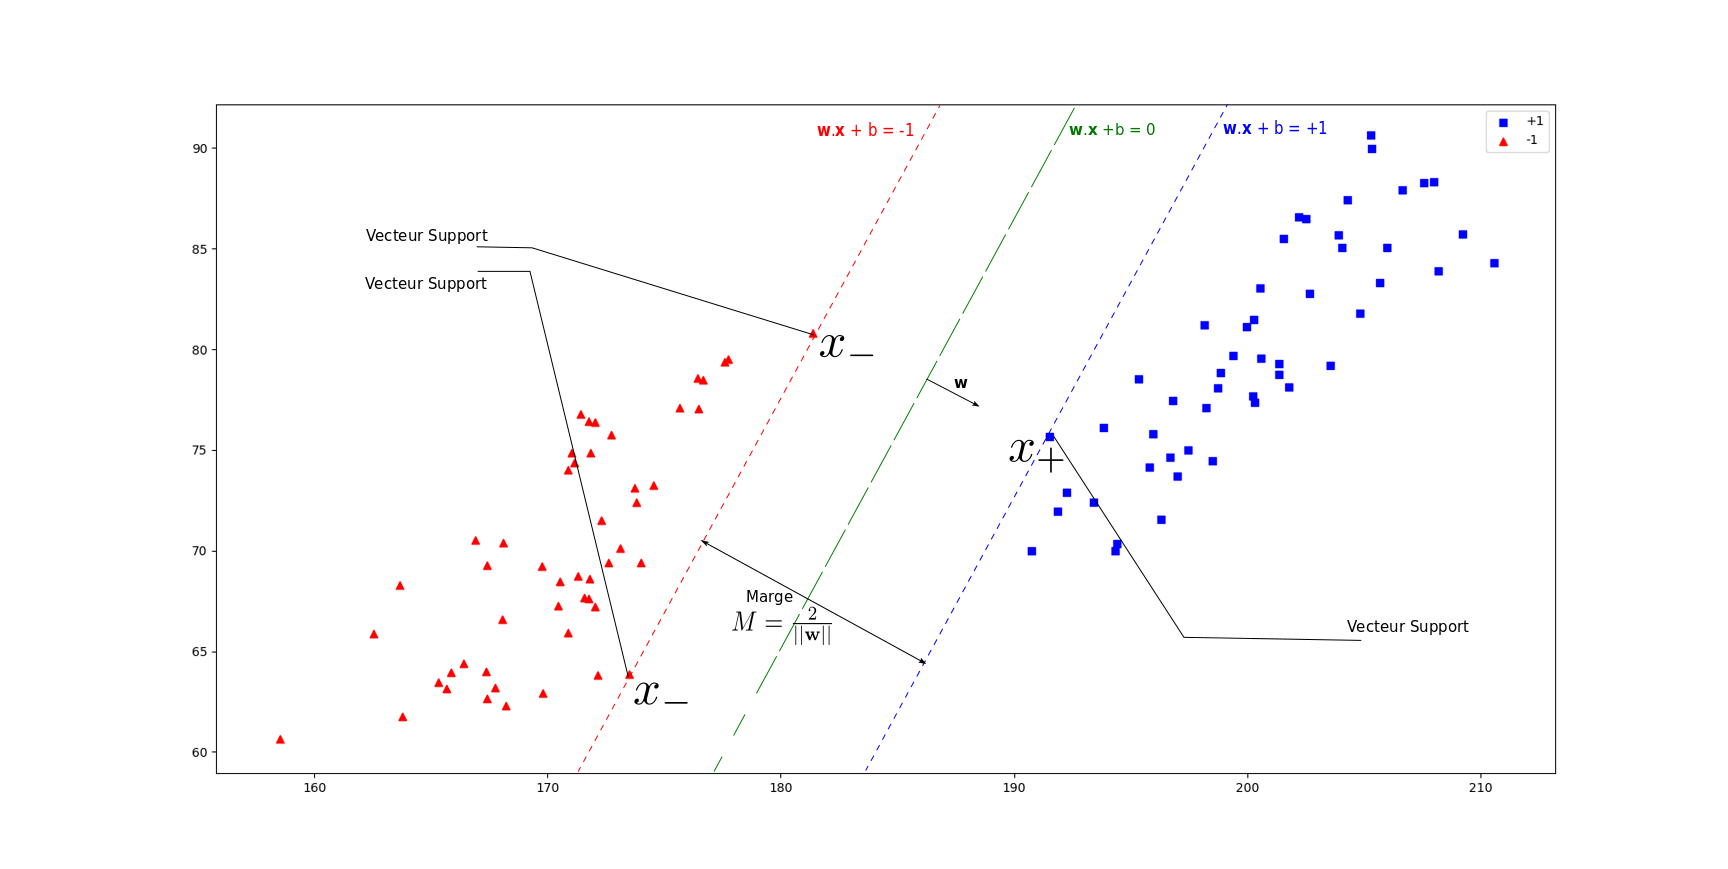
\includegraphics[width=\textwidth]{svm_margin}
			\caption{\label{fig::margin} Le séparateur linéaire SVM.}
		\end{figure}
	\end{frame}

	\begin{frame}{SVM\@: optimisation.}
		\begin{itemize}
			\item[--] On cherche à maximiser la marge:
			\begin{align}
				M &= \frac{\textbf{w}.(\textbf{x}_+ - \textbf{x}_-)}{\vert\vert \textbf{w} \vert\vert} \\
				  &= \frac{2}{\vert\vert \textbf{w} \vert\vert}
			\end{align}
			\item[--] Le problème est reformuler donc comme suit:
			\begin{equation}
				\begin{aligned}
				& \max_{\textbf{w}}
				& & \frac{2}{\vert\vert \textbf{w} \vert\vert} \\
				& \text{sous contrainte}
				& & \begin{cases}
					\textbf{w}.\textbf{X}^i + b \leq -1 & Y^i = -1 \\
					\textbf{w}.\textbf{X}^i + b \geq 1 & Y^i = 1
				\end{cases} \; \forall i = 1, \dots, n.
				\end{aligned}
			\end{equation}
			\item[--] Ou encore:
			\begin{equation}
				\begin{aligned}
				& \min_{\textbf{w}}
				& & {\vert\vert \textbf{w} \vert\vert}^2 \\
				& \text{sous contrainte}
				& & Y^i.(\textbf{w}.\textbf{X}^i + b) \geq 1 \; \forall i = 1, \dots, n.
				\end{aligned}
			\end{equation}
		\end{itemize}
	\end{frame}

	\begin{frame}{Cas non séparable.}
		\begin{figure}[H]
			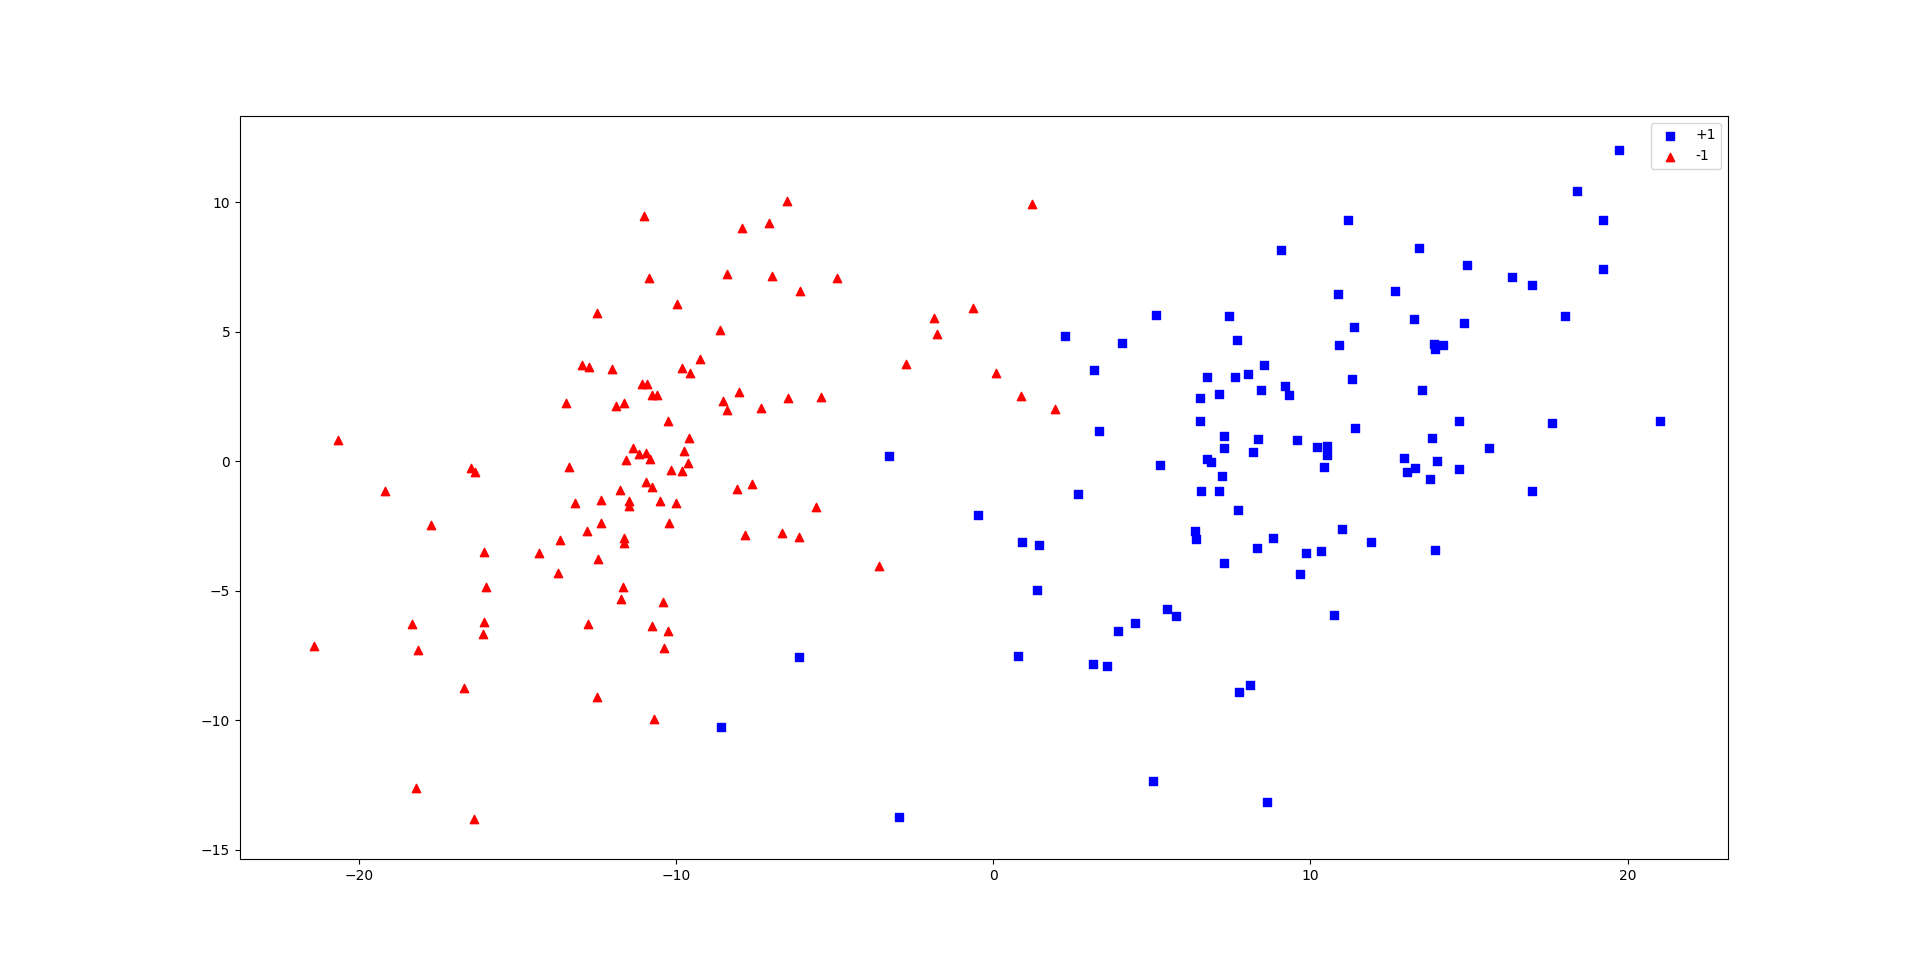
\includegraphics[width=\textwidth]{non_separable}
			\caption{\label{fig::non_sep} Le séparateur linéaire SVM.}
		\end{figure}
	\end{frame}

	\begin{frame}{Cas non séparable.}
		\begin{figure}[H]
			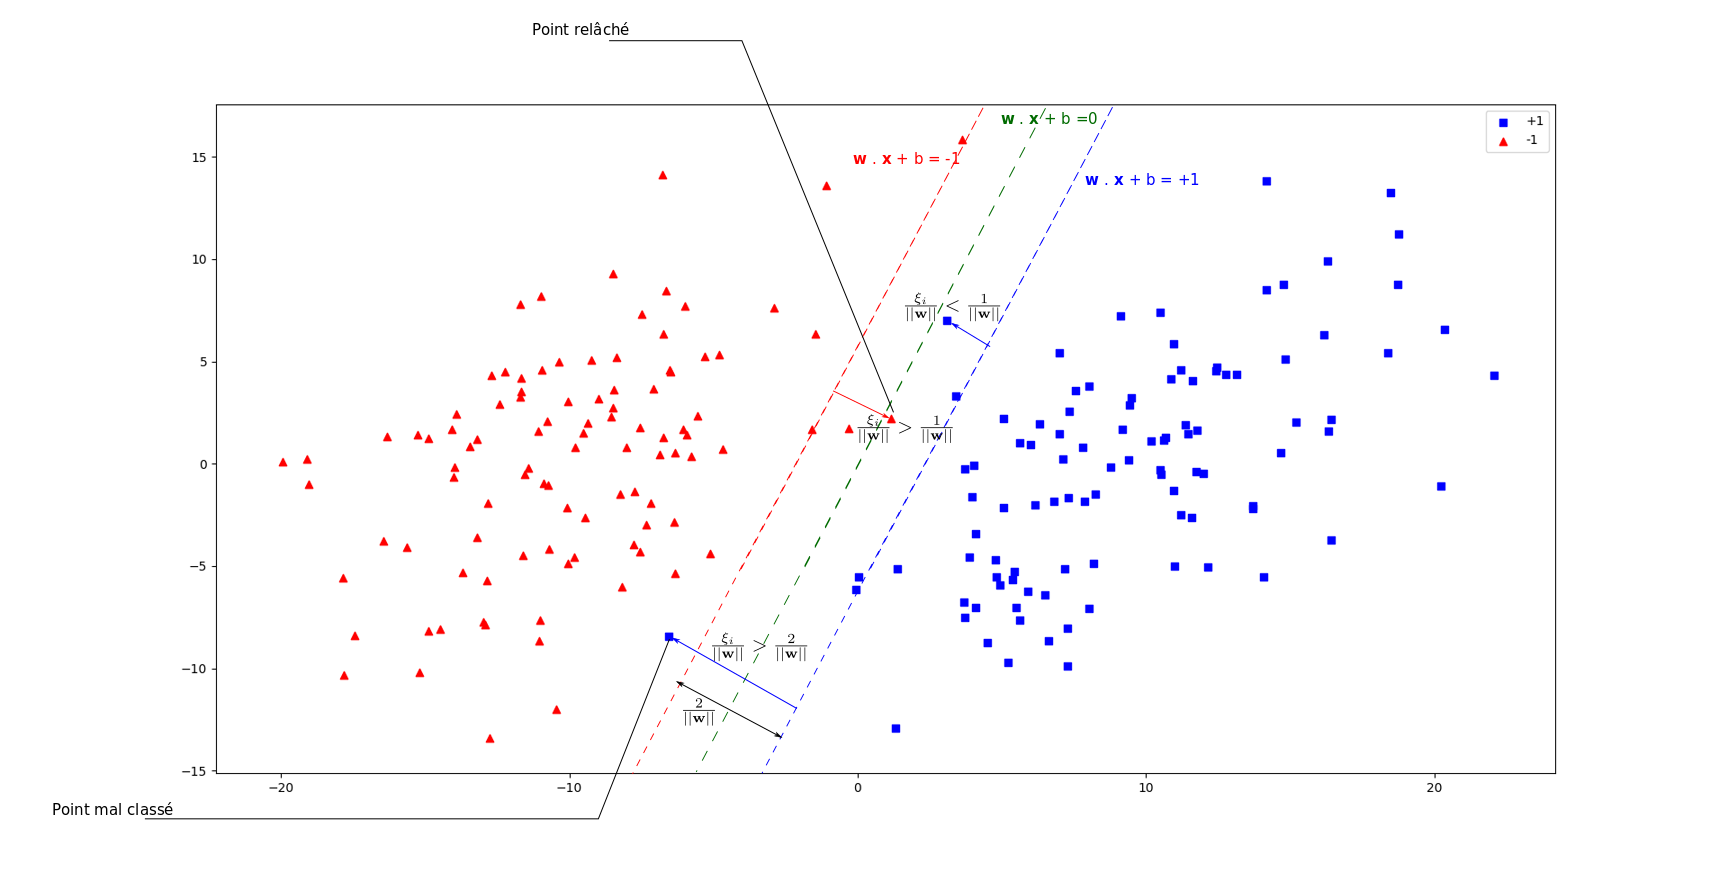
\includegraphics[width=\textwidth]{stable_margin}
			\caption{\label{fig::stable_margin} Le séparateur linéaire SVM.}
		\end{figure}
	\end{frame}

	\begin{frame}{Cas non séparable.}
		\begin{itemize}
			\item[--] Formellement on lâche du ``mou''. On accepte des fois que
			$$\exists k \; Y^k.(\textbf{w}.\textbf{X}^k + b) < 1$$
			\item[--] On peut écrire ceci autrement:
			$$\forall i=1,\dots,n \quad \exists \xi_i > 0 \quad Y^i.(\textbf{w}.\textbf{X}^i + b) \geq 1 - \xi_i$$

			\item[--] Il y a donc trois cas pour $ \xi_i $:
			\begin{itemize}
				\item[-] $\xi_i = 0 \Rightarrow$ Point bien classé;
				\item[-] $0 < \xi_i \leq 1 \Rightarrow$ Point en dehors de la marge;
				\item[-] $1 < \xi_i \Rightarrow$ Point mal classé;
			\end{itemize}

			\item[--] Dans le cas ou le problème n'est pas séparable linéairement, on peut dire donc que
			$\exists j \quad 1 < \xi_j$

			\item[--] Les différents $\xi_i$ peuvent être très grand. Il faut donc les pénaliser au moment de l'optimisation. Le problème devient donc:
			\begin{equation}
				\begin{aligned}
				& \min_{\textbf{w}, \xi_1,\dots,\xi_n \in \mathbb{R}^+}
				& & {\vert\vert \textbf{w} \vert\vert}^2 + C.\sum_{i=1,\dots,n}\xi_i\\
				& \text{sous contrainte}
				& & Y^i.(\textbf{w}.\textbf{X}^i + b) \geq 1 - \xi_i , \forall i = 1, \dots, n.
				\end{aligned}
			\end{equation}
		\end{itemize}
	\end{frame}

	\begin{frame}{Cas de $C$.}
		\begin{itemize}
			\item[--]
		\end{itemize}
	\end{frame}
	\begin{frame}{Optimization Quadratic! On peut faire mieux.}
		\begin{itemize}
			\item[--] Problème primal:
			\begin{equation}
				\begin{aligned}
				& \min_{\textbf{w}, \xi_1,\dots,\xi_n \in \mathbb{R}^+}
				& & {\vert\vert \textbf{w} \vert\vert}^2 + C.\sum_{i=1,\dots,n}\xi_i \\
				& \text{sous contrainte}
				& & Y^i.(\textbf{w}.\textbf{X}^i + b) \geq 1 - \xi_i , \forall i = 1, \dots, n.
				\end{aligned}
			\end{equation}
            \item[--] Problème dual:
            \begin{equation}
				\begin{aligned}
				& \max_{0 \leq \alpha_i \leq C ,\forall i=1,\dots,n}
				& & \sum_{i=1,\dots,n} \alpha_i - \frac{1}{2}.\sum_{l,p=1,\dots,n}\alpha_l.\alpha_p.Y^l.Y^p.(X^l.X^p)\\
				& \text{sous contrainte}
				& & \sum_{i=1,\dots,n}Y^i.\alpha_i=0
				\end{aligned}
			\end{equation}
            \item[--] Ce dernier est un problème d'optimisation linéaire qu'on sait résoudre.
		\end{itemize}
	\end{frame}
    \begin{frame}{Algorithmes en Pratiques}
		\begin{itemize}
			\item[--] Problème Primale: SGD.
            \item[--] Problème Primale: SMO et dérivées.
		\end{itemize}
	\end{frame}
	\subsection[kernel]{Kernel SVM}
	\begin{frame}{Changement d'espace}

	\end{frame}

	\begin{frame}{Kernel trick}

	\end{frame}

	\begin{frame}{Kernels Usuels}

	\end{frame}

	\section[feature selection]{Sélection d'attributs}
	\subsection[motivation]{Motivation}
	\begin{frame}{Pourquoi sélectionner les attributs?}
		Les espaces à très grande dimension ne resemble pas au plan ou au volume:
		\begin{itemize}
			\item[--]<1-> Les calculs durent plus de temps,
			\item[--]<2-> Il y a moins de volume à l'intérieur; si on compare le volume contenu dans une sphère et le volume de l'hypercube circonscrit:
			$$\frac{V(\mathbb{B}_{2}(r))}{V(\mathbb{B}_{\infty}(r))}\xrightarrow[d \to \infty]{} 0$$
			\item[--]<3-> La distance Euclidienne n'a plus de sens en très grande dimension $\longrightarrow$ moins d'attributs on a mieux sont les résultas~\cite{Domingos:2012:FUT:2347736.2347755}.
		\end{itemize}
	\end{frame}

	\begin{frame}{Comment sélectionner les attributs?}
		Encore un fois, sans connaissance préalable, la sélection d'attributs est insoluble vue le nombre exponentiel de possibilité $\sum_{k=0,\dots,n} \begin{pmatrix}
		n\\
		k
		\end{pmatrix} = 2^n$.

		On distingue donc trois types d'approche:
		\begin{enumerate}
			\item<1-> approche par filtre: on choisit les attributs en amont en reposant sur un critère,
			\item<2-> approche intégrée: on sélectionne les attributs en reposant sur les caractéristiques du classifieur,
			\item<3-> approche symbiotique: on retient les attributs les plus performants en aval.
		\end{enumerate}
	\end{frame}

	\subsection[filter approach]{Approche par filtre}
	\begin{frame}{Approche par filtre}
		\begin{itemize}
			\item[--] Corrélation: un bon sous-ensemble contient des attributs pas très corrélés entre eux $\longrightarrow$ on élimine les variables redondantes;
			\item[--] Relief: qualification d un attribut en fonction de comment ses valeurs permettent de distinguer des points qui sont proches.
		\end{itemize}
	\end{frame}

	\subsection[integrated approach]{Approche intégrée}
	\begin{frame}{Approche intégrée: cas du SVM-RFE}
		On repose par exemple sur les poids du SVM $\textbf{w}$:
		\begin{enumerate}
			\item<1-> On entraine le SVM $\longrightarrow$ on obtient le $\textbf{w}$.
			\item<2-> On choisit l'attribut $i$ avec le plus faible poids:
			$$ i \leftarrow \arg \min_{k=1,\dots,d}{\vert\vert w_k\vert\vert}$$
			\item<3-> On élimine l'attribut $i$.
		\end{enumerate}
		On procède donc par récurence jusqu'au nombre d'attributs cherché~\cite{Guyon2002}.
	\end{frame}

	\subsection[symbiotic approach]{Approche symbiotique}
	\begin{frame}{SFS}
		Sélection ascendante (SFS\@: Sequential Forward Selection).
		\begin{enumerate}
		\item<1-> On sélectionne le meilleur attribut;
		\item<2-> On lui rajoutte l'attribut qui forme la meilleur paire;
		\item<3-> On continue à rajoutter les attributs de manière à avoir à l'itération $k$ le meilleur $k$-tuple;
		\item[--]<4-> Le problème est que l'on peut ratter en procédant ainsi au meilleur ensemble.
		\end{enumerate}
	\end{frame}

	\begin{frame}{SFS}
		\begin{block}{Example}
			\begin{longtable}{c c c c c}
				\toprule
				attributs sélectionés & $1$ & $2$ & $3$ & $4$\\
				\midrule
				résultat& $0.49$ & $0.21$ & $0.19$ &$0.24$\\
				\bottomrule
			\end{longtable}
			\begin{longtable}{c c c c c c c}
				\toprule
				attributs sélectionés & $1,2$ & $1,3$ & $1,4$ & $2,3$ & $2,4$ & $3,4$\\
				\midrule
				résultat & $0.59$ & $0.51$ & $0.52$ & $0.45$ & $0.49$ & $0.48$\\
				\bottomrule
			\end{longtable}
			\begin{longtable}{c c c c c c c}
				\toprule
				attribut sélectionés & $1,2,3$ & $1,2,4$ & $1,3,4$ & $2,3,4$ & $1,2,3,4$\\
				\midrule
				résultat & $0.61$ & $0.67$ & $0.59$ & $0.78$ & $0.81$\\
				\bottomrule
			\end{longtable}
		\end{block}
	\end{frame}

	\begin{frame}{SBE}
		Sélection descendante (SBE\@: Sequential Backward Elimination).
		Cette méthode ressemble à celle d'avant.
		\begin{enumerate}
		\item<1-> On élimine le attribut qui ne rapporte pas beaucoup;
		\item<2-> On réitère de façon à ce que qu'à l'itération $k$ on aura éleminé les $k$ pire attribut;
		\item<3-> On continue jusqu'à ce qu'il ne reste plus qu'un attribut ou un nombre donné.
		\item[--]<4-> On rencontre le même problèmes qu'avant.
		\end{enumerate}
	\end{frame}

	\begin{frame}{Comment résoudre le problème donc?}
		\begin{itemize}
			\item<1-> Combinaison SFS + SBE\@: sélection Plus-L-Moins-R\@:
			\begin{itemize}
				\item Si $L > R$, on commence avec un ensemble vide, on ajoute L attributs puis on en enlève R\@,
				\item Si $L < R$, on commence avec tous les attributs, on enlève R attributs puis on en rajoute L\@;
			\end{itemize}
			\item<2-> On garantit la convergence vers une solution unique:
			\begin{itemize}
				\item On peut vérifier que SFS et SBE ne se contredisent pas.
				\item On peut procéder comme dans l'example:
				\begin{block}{Example}
					Si SFS veut ajouter un attribut, il vérifie qu'il n'a pas été éliminé par SBE\@. Si oui, il prend le 2$^{\text{ème}}$ meilleur et ainsi de suite.
				\end{block}
			\end{itemize}
		\end{itemize}
	\end{frame}

	\section*{References}
	\begin{frame}[allowframebreaks]{References}
		\nocite{sklearn_api}
		\bibliographystyle{apalike}
		\bibliography{references.bib}
	\end{frame}

	%%%%%%%%%%%%%%%%%%%%%%%%%%%%%%%%%%%%%%%%%%%%%%%%%%%%%%%%%%%%%%%%%%%%%%%%%%%%%%%%%%%%%%%%%%%%%%%%%%%%%%%%%
	\usebackgroundtemplate{
		\begin{tikzpicture}
			\draw (0,0.5) node[right] { 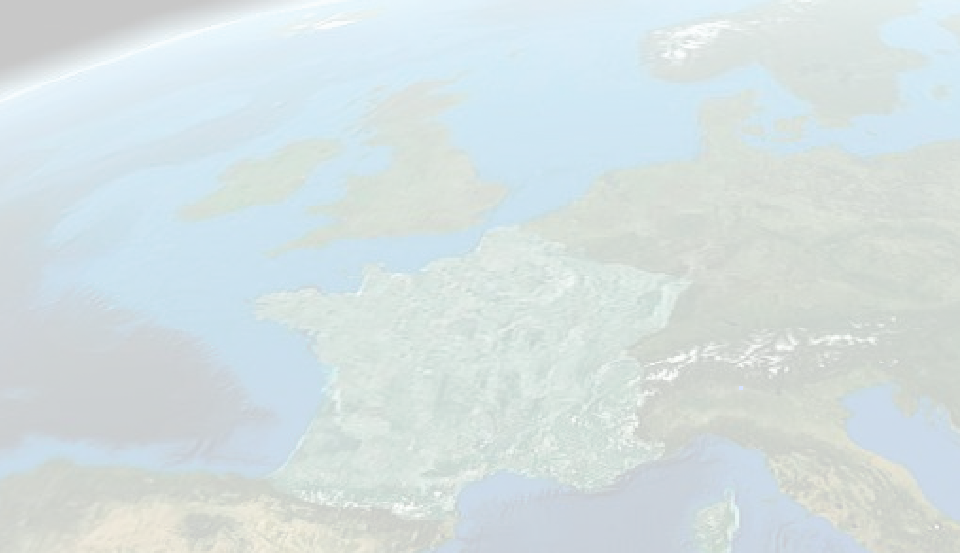
\includegraphics[width=12.5cm]{from_space_background} };
			\draw (0,5) node[right] { 
\includegraphics[height=1.5cm]{ign_logo} };
			\draw (1.5,4.95) node[right] { 
\includegraphics[width=3cm]{ign_logo_bottom} };
		\end{tikzpicture}
	}
	\begin{frame}[plain,c]
		\vspace{3cm}
		
\begin{tikzpicture}
			\draw (0,0)node{};
			\draw (4.5,1) node[color =IGNGris, inner sep=0.5em, minimum size=0.5em, text centered,font=\LARGE] { Thanks for your attention, };
			\draw (4.5,0) node[color =IGNGris, inner sep=0.5em, minimum size=0.5em, text centered,font=\LARGE] { I am ready for your questions! };
			\draw (4.5,-2) node[color =IGNVert, inner sep=0.5em, minimum size=0.5em, text centered,font=\LARGE] { oussama.ennafii@ign.fr };
		\end{tikzpicture}
	\end{frame}
\end{document}
